\section{Membuat Penomoran Referensi}
Untuk menambahkan referensi atau melakukan sanitasi pada latex kita dapat menggunakan berbagai macam cara. Salah satu cara sederhana yang dapat kita gunakan adalah dengan menggunakan environment yang di sebut \textit{thebibliography}. Namun, kebanyakan orang saat ini menggunakan \textit{BibTeX} untuk melakukan sanitasi sebagai acuan referensi. Dengan menggunakan \textit{BibTex} kita dapat mengatur sitasi sendiri secara terpisah dalam format file \*.bib \cite{atmaja2015tutorial}. Disaat mengutip maupun menggunakan sanitasi diperkenankan untuk memberi keterangan referensi atau sumber asal suatu kutipan dan gagasan. Untuk mengetahui bagaimana menambahkan referensi pada latex, kita dapat melihat langkah-langkahnya seperti pada gambar \ref{fig:contohpenomoranref}.
\begin{figure}[!htbp]
  \centering
  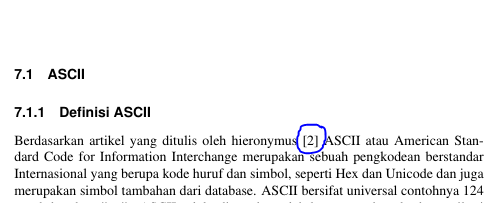
\includegraphics[width=.75\textwidth]{figures/contohpenomoranref.png}
  \caption{Ini adalah Contoh Penomoran Referensi}\label{fig:contohpenomoranref}
\end{figure}
\par Bagaimana cara membuatnya di Latex? berikut cara membuatnya:
\begin{enumerate}
  \item Cari materi yang akan dikutip melalui Google Scholar seperti pada gambar \ref{fig:scholar} ,
  \begin{figure}[!htbp]
  \centering
  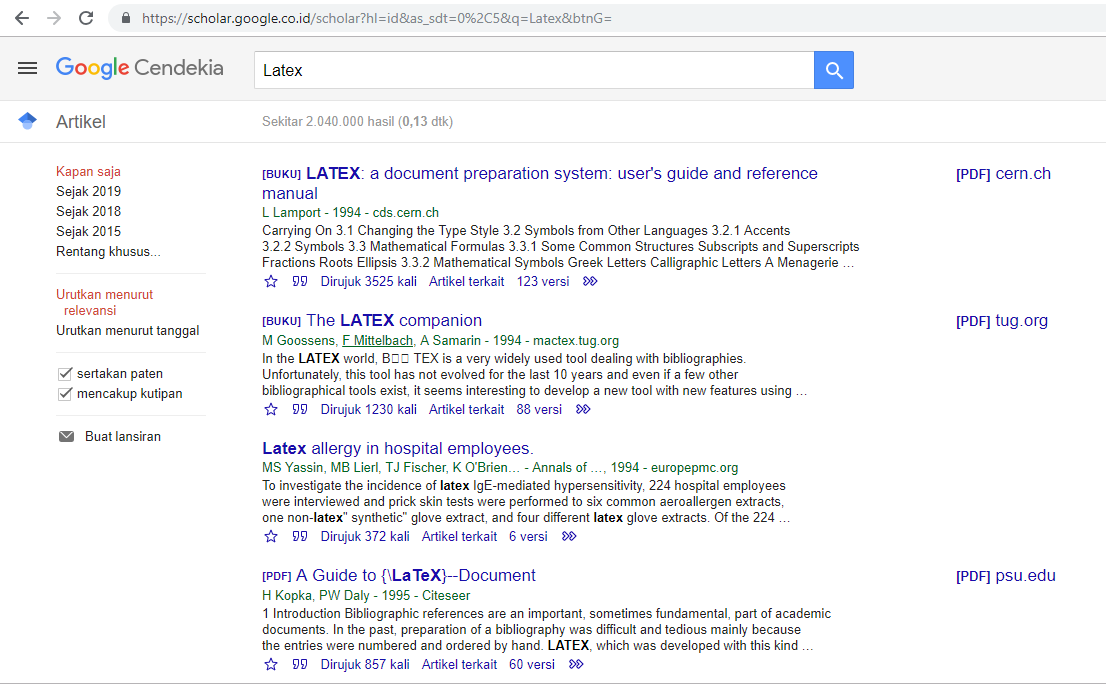
\includegraphics[width=.75\textwidth]{figures/scholar.png}
  \caption{Ini adalah Halaman Google Scholar}\label{fig:scholar}
\end{figure}
  \item Setelah selesai mengutip jangan lupa untuk mengambil script bibtexnya dengan cara klik pada tanda kutip seperti pada gambar \ref{fig:awalbibtex},
  \begin{figure}[!htbp]
  \centering
  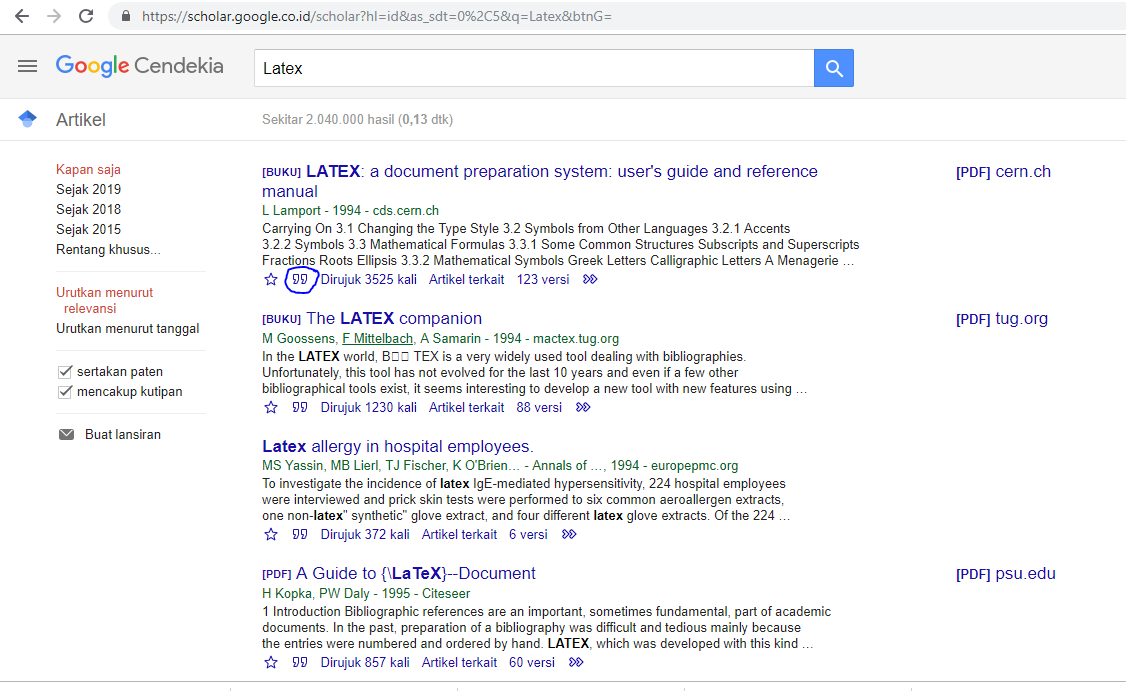
\includegraphics[width=.75\textwidth]{figures/awalbibtex.png}
  \caption{Ini adalah Tanda proses awal mengambil reference}\label{fig:awalbibtex}
\end{figure}
  \item Maka akan muncul seperti gambar \ref{fig:kutip}, lalu pilih Bibtex.
  \begin{figure}[!htbp]
  \centering
  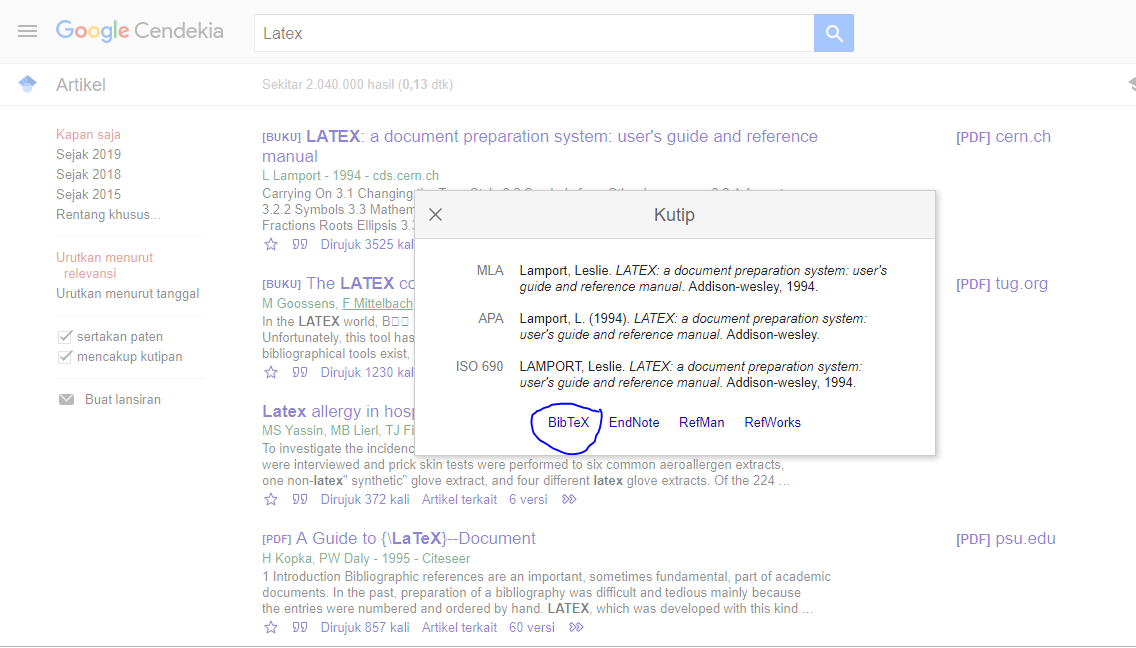
\includegraphics[width=.75\textwidth]{figures/kutip.png}
  \caption{Ini adalah Pilihan mengutip}\label{fig:kutip}
\end{figure}
  \item Setelah memilih Bibtex maka akan muncul script seperti pada gambar \ref{fig:scriptbibtex},
  \begin{figure}[!htbp]
  \centering
  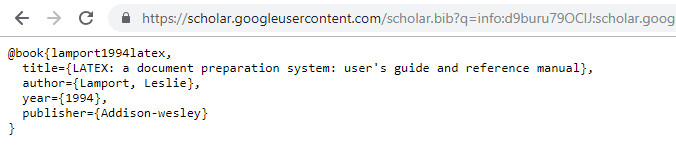
\includegraphics[width=.75\textwidth]{figures/scriptbibtex.png}
  \caption{Ini adalah Script BibTex}\label{fig:scriptbibtex}
\end{figure}
  \item Script tersebut dicopy pada direktori yang dikerjakan, khususnya pada bagian reference.bib seperti pada gambar \ref{fig:direktori} dan \ref{fig:reference} pada editor,
  \begin{figure}[!htbp]
  \centering
  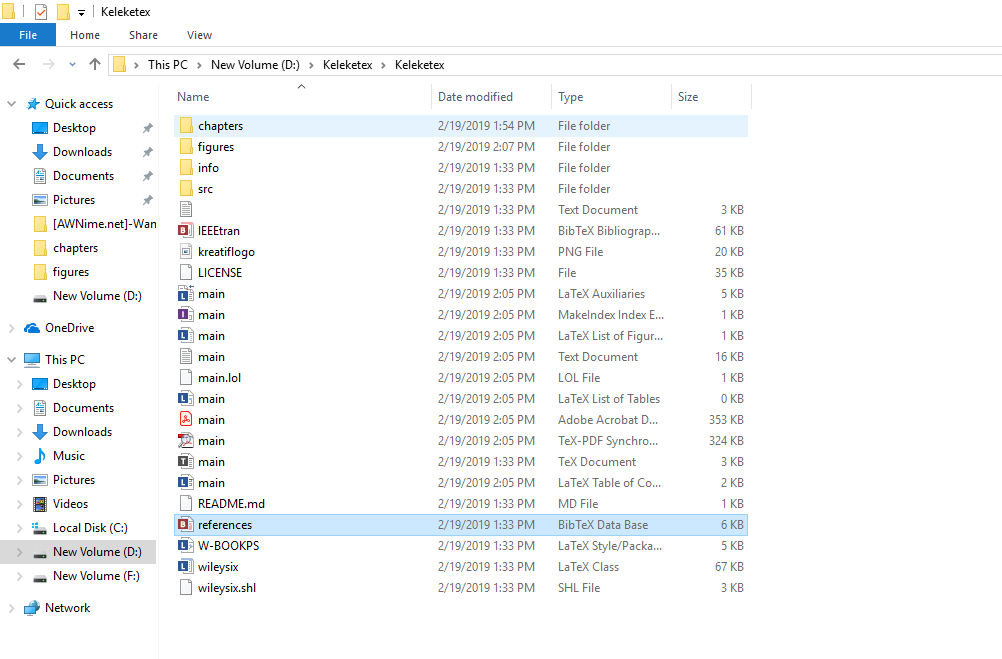
\includegraphics[width=.75\textwidth]{figures/direktori.png}
  \caption{Ini adalah Direktori pekerjaan}\label{fig:direktori}
\end{figure}
\begin{figure}[!htbp]
  \centering
  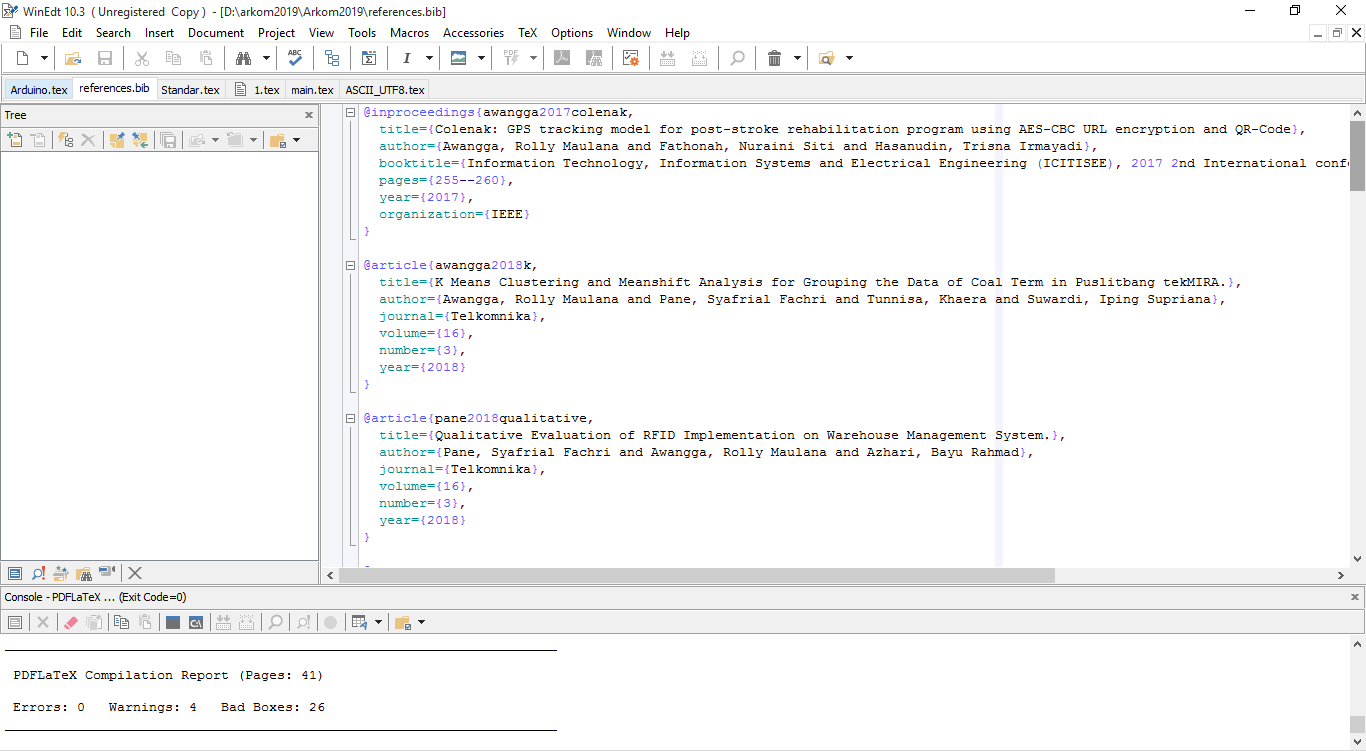
\includegraphics[width=.75\textwidth]{figures/reference.png}
  \caption{Ini adalah Reference.bib}\label{fig:reference}
\end{figure}
  \item Setelah dicopy, jangan lupa disave.
  \item Buka kembali pada lembar kerja yang sudah diberi kutipan/gagasan. Lalu tambahkan script listing \ref{lst:capaian}. setelah kutipan maka akan muncul seperti pada gambar \ref{fig:memilihsumber},
\lstinputlisting[caption=Penggunaan perintah cite untuk reference,label={lst:capaian}]{src/1/reference.tex}
  \begin{figure}[!htbp]
  \centering
  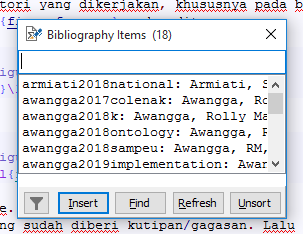
\includegraphics[width=.75\textwidth]{figures/memilihsumber.png}
  \caption{Ini adalah Proses pemilihan sumber}\label{fig:memilihsumber}
\end{figure}
  \item Pilih insert dan save.
  \item Untuk proses compilenya dilakukan 2 kali yaitu pada main.tex pilih Tex lalu pilih pdflatex dan Bibtex, dilakukan berulang minimal 3 kali compile. Seperti pada gambar \ref{fig:pdflatex} untuk pdflatex dan \ref{fig:bibtexx} untuk BibTex.
   \begin{figure}[!htbp]
  \centering
  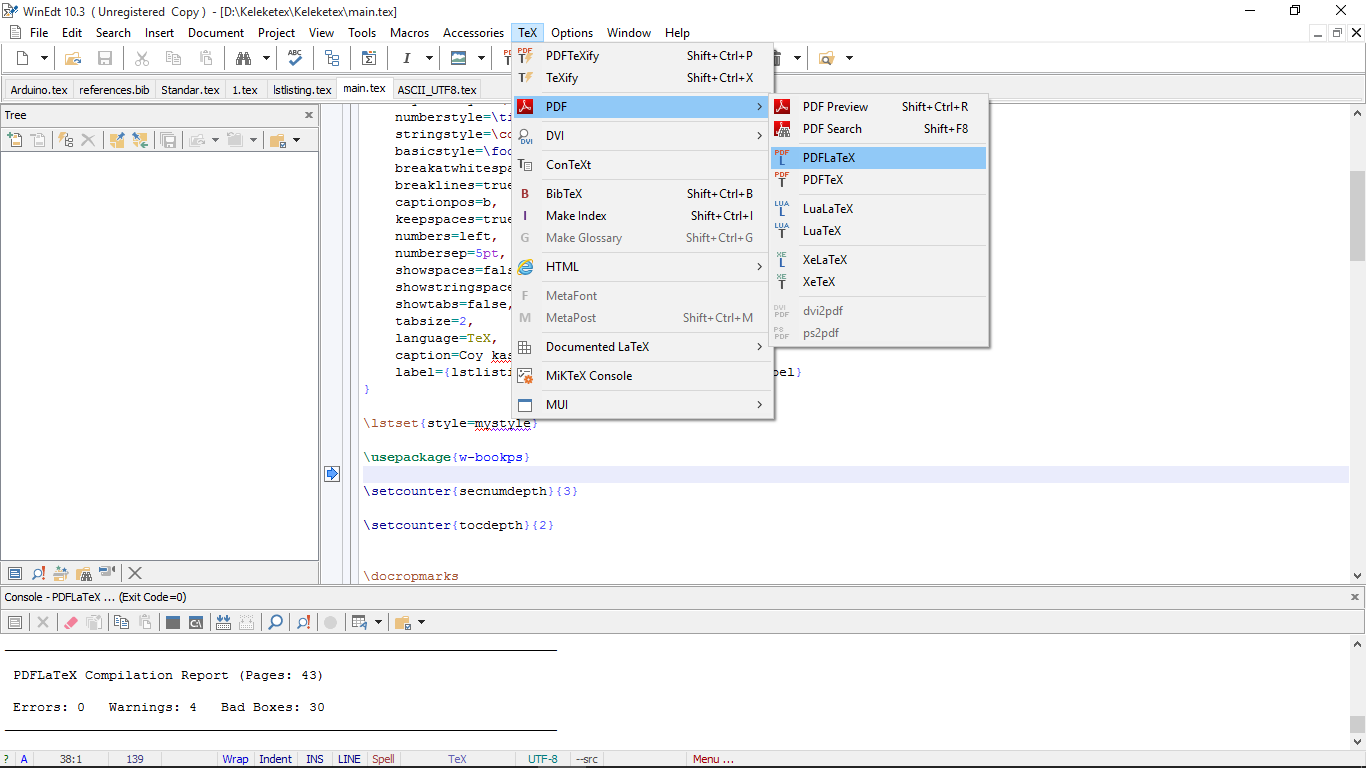
\includegraphics[width=.75\textwidth]{figures/pdflatex.png}
  \caption{Ini adalah Compile pdflatex}\label{fig:pdflatex}
\end{figure}
   \begin{figure}[!htbp]
  \centering
  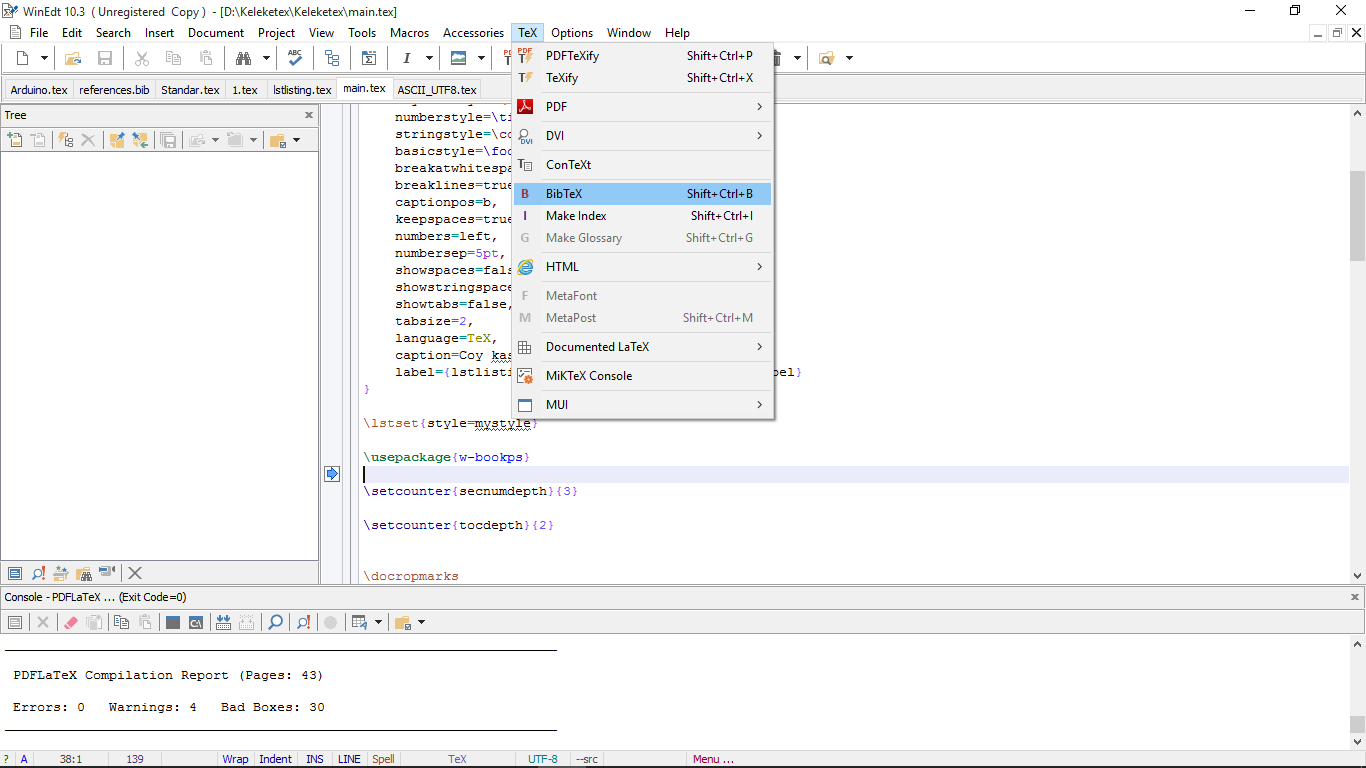
\includegraphics[width=.75\textwidth]{figures/bibtexx.png}
  \caption{Ini adalah Compile BibTex}\label{fig:bibtexx}
\end{figure}
\end{enumerate}

